% last updated in April 2002 by Antje Endemann
% Based on CVPR 07 and LNCS, with modifications by DAF, AZ and elle, 2008 and AA, 2010, and CC, 2011

\documentclass[runningheads]{llncs}
\usepackage{graphicx}
\usepackage[font=small]{caption}
\usepackage{subcaption}
\captionsetup{compatibility=false}
\usepackage{amsmath,amssymb} % define this before the line numbering.
\usepackage{ruler}
\usepackage{color}
\usepackage{url}
\usepackage{comment}
\usepackage[width=122mm,left=12mm,paperwidth=146mm,height=193mm,top=12mm,paperheight=217mm]{geometry}
\usepackage{multirow}
\usepackage{tabularx}
\newcolumntype{Y}{>{\centering\arraybackslash}X}
\captionsetup[table]{belowskip=12pt,aboveskip=4pt}
\setlength{\floatsep}{7pt plus 2pt minus 2pt}
\setlength{\textfloatsep}{7pt plus 2pt minus 2pt}
\setlength{\intextsep}{7pt plus 2pt minus 2pt}

\begin{document}
% \renewcommand\thelinenumber{\color[rgb]{0.2,0.5,0.8}\normalfont\sffamily\scriptsize\arabic{linenumber}\color[rgb]{0,0,0}}
% \renewcommand\makeLineNumber {\hss\thelinenumber\ \hspace{6mm} \rlap{\hskip\textwidth\ \hspace{6.5mm}\thelinenumber}}
% \linenumbers \

\pagestyle{headings}
\mainmatter
\def\ECCV14SubNumber{150}  % Insert your submission number here

\title{A Motion Blur Resilient Fiducial Marker For Quadcopter Imaging} % Replace
% with your title

\titlerunning{ECCV-14 submission ID \ECCV14SubNumber}

\authorrunning{ECCV-14 submission ID \ECCV14SubNumber}

\author{Anonymous ECCV submission}
\institute{Paper ID \ECCV14SubNumber}

\maketitle

\begin{abstract}
This paper describes the design and evaluation of a binary fiducial marker
for use with low-cost quadcopters.  Fiducial markers are commonly placed
in environments to provide a uniquely identifiable object in the scene.
For quadcopter applications, fiducials are
typically used for evaluating planning algorithms by allowing ground truth
positions in the scene to be detected from the quadcopter's camera. Quadcopters,
however, are subject to quick and unstable motions that can cause significant motion
blur that severely affects the detection rate of existing fiducial markers.
This problem motivated us to design a fiducial that is robust to motion blur.
Our proposed fiducial design uses concentric circles with the observation that
the direction perpendicular to the motion blur direction will be unaffected by
the blur.  As a result, the fiducial code along this direction is recognizable.
The circular design allows this to work for all motion blur directions.  We
detail the design and detection algorithm for our fiducial and show that our
marker can significantly outperform existing fiducial markers in scenes captured with a quadcopter.
\keywords{Fiducials, tracking, recognition under blur}
\end{abstract}

\section{Introduction}

The recent availability of low-cost quadcopters has help to fuel significant efforts in
research focused on unmanned aerial vehicles.  Navigation and planning of
these vehicles is typically performed using onboard inertial sensors and/or
vision based modules that uses visual cues in the real world~\cite{Davison:2007}.
However, to evaluate the effectiveness of navigation methods, artificial
fiducial markers are commonly placed into the environment to provide
additional information that serves for ground-truth
positional measurements (e.g.,\cite{Bosnak:2012,Lim09,Klopschitz:2007}).

In order to be effective, fiducial markers (or simply, fiducials) need
to be easily detected in the scene.  A variety of fiducial markers
have been proposed in the literature
(e.g.,~\cite{NaimarkF02,ARToolkit02,Fiala05,Pitag13,runetag11}).
These take the form of binary codes arranged into rectangular grids (\cite{ARToolkit02,Fiala05})
or other geometric features arranged in predefined spatial patterns
(\cite{NaimarkF02,Pitag13,runetag11}).
Figure \ref{fig:teaser}-top shows an example of the popular ARTag\cite{Fiala05} as
seen from a quadcopter.  A problem for existing fiducials is  that low-cost quadcopters
often exhibit very quick and erratic physical movements that
results in motion blur in the quadcopter's onboard camera.  This motion blur has
an adverse effect on the  recognition of fiducial  markers.  This can be seen in
Figure \ref{fig:teaser}(top) where the ARTag cannot be recognized due to motion
blur. This is not too surprising as most  existing fiducials are not explicitly
designed to handle motion blur.

Compounding this problem is the additional issue of dropped video frames from
the quadcopter's wireless communication module.   This means that not only is blurring
introduced, but there may be large discontinuities in the patterns position due
to missing video frames.  As we will show in Section 4, this later problem
makes it challenging to apply tracking algorithms that can exploit temporal
coherence for determining the fiducial positions.

\noindent\textbf{Contribution:}~~To address these problems, we propose a
fiducial that is designed to be robust to motion blur.  Our design is based on
concentric circles as shown in Figure \ref{fig:teaser}-b.  The design is based
on the observation that motion blur from a quadcopter tends to be linear in
nature.  As such, when our code is blurred, there is no blur in the direction
perpendicular to the direction of motion.   This allows the signature of the
fiducial to remain intact in any direction.  In addition, by using concentric
rings, we can treat the presence or absence of a ring as a bit, allowing us to
assign an code to the marker.  Our experiments show that this design can
significantly outperform existing codes in the face of motion blur. As far as
we are aware, this is the first work to propose a blur resistant marker.

The remainder of this paper is organized as follows.   Section 2 gives an
overview of related work, focused on fiducials as well as the related problem of
tracking.  Section 3 discusses the our design and detection algorithm, by first
examining the performance of existing codes under blur. Section 4 shows several
experiments using quadcopter imagery.  This is followed by a discussion and
summary in Section 5 and 6 respectively.

\begin{figure}
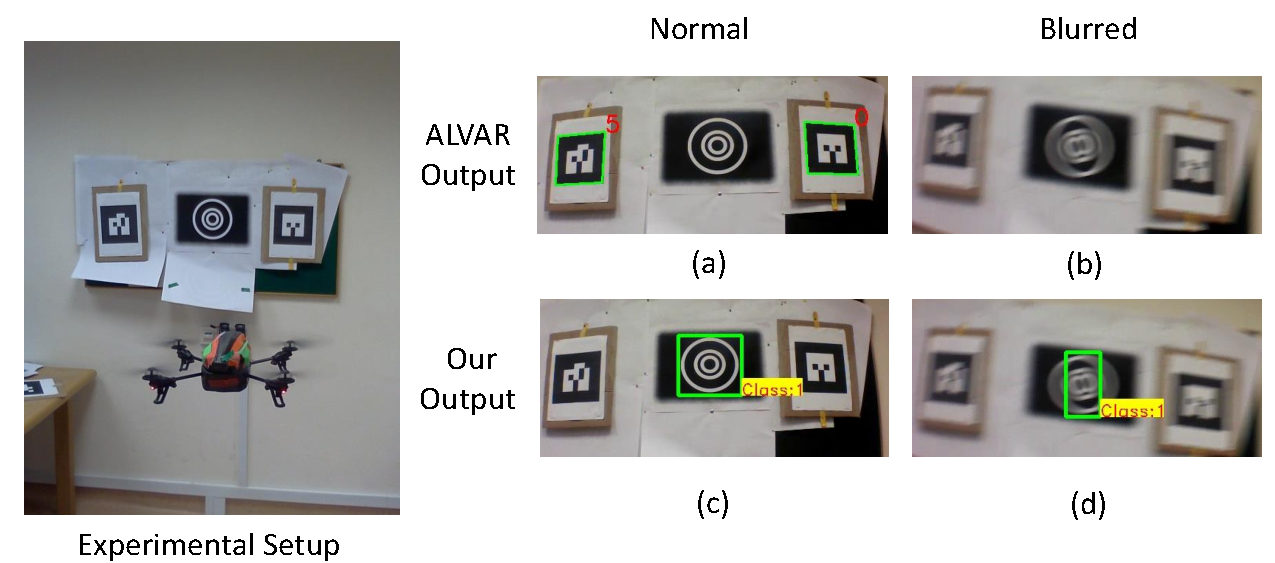
\includegraphics[width=\linewidth]{teaser.pdf}
\caption{This figure shows experimental setup and comparison of
output of ALVAR\cite{alvar} (for detecting ARTag) versus our blur resistant fiducial
in a normal and blurred scene. The scene contains two ARTags and our code.
(a) shows that the ARTag can be detected when the image has no blur. 
(b) shows that ARTags are no longer detectable due to the blur.
(c-d) show the same images in (a) and (b) where our code is being detected.}
\label{fig:teaser}
\end{figure}

\section{Related Work}

Our work is related to two areas: fiducial markers and object tracking. We will
briefly discuss work done in both areas.

\begin{figure}
 \begin{subfigure}[b]{0.19\textwidth}
  \centering
  
\includegraphics[width=\linewidth]{intersense.jpg}
  Intersense\cite{NaimarkF02}
 \end{subfigure}
 \begin{subfigure}[b]{0.19\textwidth}
 \centering
  
\includegraphics[width=\linewidth]{pattKanji.pdf}
  ARToolkit\cite{ARToolkit02}
 \end{subfigure}
 \begin{subfigure}[b]{0.19\textwidth}
  \centering
  
\includegraphics[width=\linewidth]{ARtag.jpg}
  ARTag\cite{Fiala05}
 \end{subfigure}
 \begin{subfigure}[b]{0.19\textwidth}
  \centering
  
\includegraphics[width=\linewidth]{pifiducial.jpg}
  Pi-Tag\cite{Pitag13}
 \end{subfigure}
 \begin{subfigure}[b]{0.19\textwidth}
  \centering
  
\includegraphics[width=\linewidth]{our_fiducial}
  Our Fiducial
 \end{subfigure}
 \caption{This figure shows the design of several existing fiducial markers.  While
 suitable for many environments that are not designed to be recognized under blur.}
 \label{fig:previous_work}
\end{figure}

\noindent{\textbf{Fiducials:}}~Figure~\ref{fig:previous_work} shows several 
examples of existing fiducial markers.  Many designs use a two dimensional
barcode inside a rectangular grid. One of the examples of such fiducial is,
ARToolkit\cite{ARToolkit02}, well known toolkit in Augmented Reality (AR)
system. Kato et al.\cite{kato-artoolkit} have demonstrated the use of ARToolkit
to find the pose in video based AR conferencing system. Many AR applications
used ARToolkit due to its simplicity and efficiency.

Fiala et al. \cite{Fiala05} developed a fiducial termed, ARTag, which is a
bi-tonal system consisting of a square border and an interior region filled
with a 6x6 grid of black or white cells. The improvement in ARTag compared to
ARToolkit was detection of corners instead of detection of lines to find
possible pattern. It proved to be more efficient than \cite{ARToolkit02} in
terms of marker recognition rate as well as the number of different patterns
which can be created. But, drawback of ARTag is, under significant amount of
motion blur, corners can not be detected, resulting in non-recognition of tag.

There were also attempts to use circular patterns instead of rectangular, as
the projective transformation of circles, i.e., conics, are invariant with
respective to point of view of camera\cite{runetag11}. Also, such patterns are
more distinguishable from the background scene due to their unique design. 

The use of concentric rings was used  by Gatrell et al.\cite{concentric}
for monocular pose estimation as well as object identification in space. Cho et al.
\cite{Cho:2001,Cho97fastcolor} have used multicolor rings instead of
black and white rings\cite{concentric} to increase possible number of fiducials.
These multicolor rings are used in wide area tracking in large scale
applications. 

Naimark et al. \cite{NaimarkF02} have combined concentric rings and 2D bar code
in their fiducial named, Circular Data Matrix. It was beneficial in terms of
easy detection of fiducial as well as being able to encode more unique IDs.  

All of these fiducials are not recognizable under occlusion.
Bergamasco et al. \cite{runetag11} have divided fiducial into number of
circular dots, and arranged them in circular fashion, named as RUNE-Tag.
RUNE-tags are reportedly detectable even if 50\% of fiducial area is occluded.
Bergamasco et al. have developed another fiducial, named as Pi-Tag
\cite{Pitag13}, using the cross-ratio concept. As cross-ratio is projective
invariant, the detection of Pi-tag is easier than other tags. Also, compared
to RUNE-tag, it uses remarkably less number of circular dots (12 dots instead of
minimum of 43 dots), still recognisable under occlusion.

But again problem with circular fiducials is, it is very difficult to detect
ellipses accurately under significant motion blur. So, under blur, recognition
rate of these fiducials is very low.

Zhang et al.\cite{Zhang:2002} and Claus et al. \cite{ClausF04} have done
quite comprehensive comparative study of various fiducial marker systems with
respect to processing time, recognition rate and accuracy with
respect to viewing angle and distance.

\noindent{\textbf{Tracking:}}~~Fiducial detection between successive video 
frames can be considered a tracking problem where the tracked object is fiducial itself.
There is a very large body of research dedicated to tracking and interested
readers are referred to~\cite{Yilmaz:2006} for a survey.

Most tracking methods( \cite{Ross:2008,Wu:2009,Perez02,Mei:2009} ) assume the
image sequence to be blur free. In reality, however, motion blur in video
sequences is often unavoidable. Wu et al.\cite{Wu:2011} have developed
BLUr-driven Tracker (BLUT) framework for tracking motion-blurred targets. BLUT
is based on the observation that although motion blurs degrade the visual
features of the target, they at the same time, provide useful cues about the
movements to help tracking.

The BLUT framework successfully tracks blurred target when there is uniform motion
and the position of tracked object does not change drastically in successive
frames. But as we will demonstrate in Section 4, the erratic motion from quadcopters as 
well as the problem of dropped video frames is beyond the current ability of such trackers.

\section{Design of Fiducial}

We begin by first motivating the need for a new blur resistant fiducial by examining
the performance of prior fiducials under motion blur.  After this, we detail
our design as well as the detection algorithm used to find our marker in an image.

\subsection{Examining Prior Fiducials Under Motion Blur}

Before we detail the design of our fiducial, we examine the performance of two
popular fiducials under motion blur.  Specifically we examine ARTags
\cite{Fiala05} and PiTags\cite{Pitag13} given their difference in geometry design.

To simulate the appearance of the maker as seen by a quadcopter,  we scaled down
ARTag as well as PiTag fiducial to size 150x150. Both fiducials are then blurred
at various orientations with different blurs scales (denoted in pixels).   The
blur motion ranged from 15 to 50 in magnitude, representing small to significant
motion blur. Figure \ref{fig:artag_pitag} shows the visual appearance of the
blurred tags. We then try to detect the markers using the ALVAR
library\cite{alvar} and Pi-Tag library\cite{ros_pitag}.
The table in the left side of Figure
\ref{fig:artag_pitag} shows the recognition rate (in percent) of two fiducial
markers at various blur scales under different orientation.   As we can see,
the PiTag performance quickly diminished under small amounts of blur, however,
at 35 motion blur, ARTag is recognition rate drops to less than 20\%.

\noindent\begin{minipage}[h!]{\textwidth}
\noindent\begin{minipage}{0.6\textwidth}
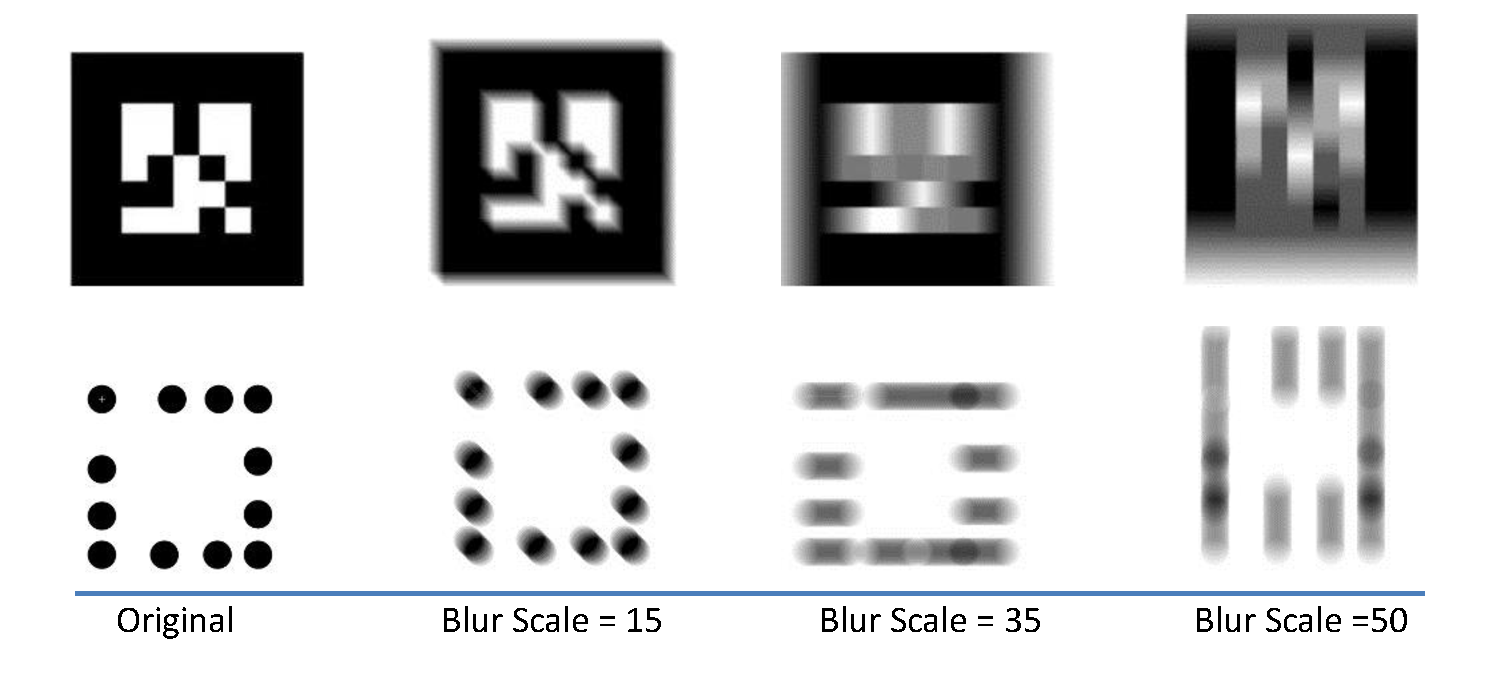
\includegraphics[width=\textwidth]{artag_pitag.pdf}
%\captionof{figure}{Blurred AR Tag and Pi--tag with various blur scales}
\end{minipage}
\begin{minipage}{0.35\textwidth}
%\captionof{table}{Recognition rate of AR Tag and Pi-tag fiducial marker atvarious blur scales}
\begin{tabularx}{\textwidth}{|Y|Y|Y|}
\cline{1-3}
\small{Blur} & \multicolumn{2}{c|}{ \small{Recognition Rate}}
\\\cline{2-3}
\small{Scale}& \small{AR Tag} &	\small{Pi-Tag} \\ \cline{1-3}
\small{15} & \small{100} & \small{100} \\ %\cline{1-3}
\small{30} & \small{0} & \small{100} \\  %\cline{1-3}
\small{35} & \small{0} & \small{19} \\ %\cline{1-3}
\small{50} & \small{0} & \small{0} \\ \cline{1-3}
\end{tabularx}
\end{minipage}
\label{fig:artag_pitag}
\captionof{figure}{Figure showing ARTag and Pi-tag blurred with various blur
scales at different orientation. Table on the right shows the recognition rate
(in percent) of both fiducial markers at various blur scales along all blur
orientations.  Recognition rates for both tag is significantly reduced due to
blur.
For severe blur, detection is not possible.}
\end{minipage}

\subsection{Blur Resistant Fiducial}

\begin{comment}

\begin{minipage}{\textwidth}
  \begin{minipage}[b]{0.49\textwidth}
\captionof{table}{Recognition rate of AR Tag at various blur scales}
\centering
 \begin{tabularx}{0.75\textwidth}{|Y|Y|}
\cline{1-2}
Blur Scale & Recognition Rate(\%) \\ \cline{1-2}
30 & 100\\ \cline{1-2}
35 & 19 \\ \cline{1-2}
40 & 9 \\ \cline{1-2}
45 & 5 \\ \cline{1-2}
50 & 0 \\ \cline{1-2}
\end{tabularx}
\label{tab:ARTag_blur}
 \end{minipage}	
 \begin{minipage}[b]{0.49\textwidth} 	
\captionof{table}{Blur angle range}
\centering
\begin{tabularx}{0.75\textwidth}{|Y|Y|}
\cline{1-2}
Blur Scale & Blur Angle Range \\ \cline{1-2}
30 & 0 -- 90\\ \cline{1-2}
35 & 32 -- 58 \\ \cline{1-2}
40 & 41 -- 48 \\ \cline{1-2}
45 & 41 -- 48 \\ \cline{1-2}
50 & 44 -- 46 \\ \cline{1-2}
\end{tabularx}
\label{tab:artag_blurangle}
 \end{minipage}
\end{minipage}

From Table \ref{tab:ARTag_blur}, it can be clearly seen that performance of
ARTag drastically degrade with increase in blur scale.

We have also analysed the recognition rate along different blur orientations
(from 0 to 90 degrees) at different blur scales. We found that per blur scale,
at certain blur orientations, recognition of ARTag fails. Table shows the range
of blur angles for which we are able to recognise the ARTag at different blur
scales. From Table \ref{tab:artag_blurangle}, it can be seen that, when blur
scale is greater than 30, ARTag is not recognisable with horizontal blur
orientation(blur angle near zero degrees) as well as vertical blur
orientation(blur angle near 90 degrees).

We have performed blur simulation experiment on Pi-tag \cite{Pitag13} to find
how blur effects circular patterns. We tried to detect blurred Pi-tag using
\cite{ros_pitag}.

\begin{figure}
\begin{subfigure}[b]{0.3\textwidth}
  \centering
  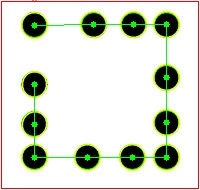
\includegraphics[width=\linewidth]{detect_noblur.jpg}
  No Blur
 \end{subfigure}
 \begin{subfigure}[b]{0.3\textwidth}
  \centering
  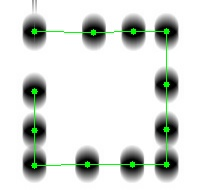
\includegraphics[width=\linewidth]{detect_blur15.jpg}
  Blur Scale = 15
 \end{subfigure}
 \begin{subfigure}[b]{0.3\textwidth}
  \centering
  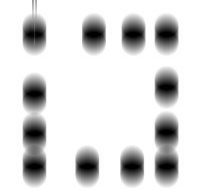
\includegraphics[width=\linewidth]{nodetect_blur20.jpg}
  Blur Scale = 20
 \end{subfigure}
 \caption{Effect of blur on detection of Pi-Tag}
 \label{fig:pitag_blur}
\end{figure}

From Figure \ref{fig:pitag_blur}, it can be seen that, Pi-tag detection
fails when blur scale is more than 15. The reason behind this is, Pi-tag
detection is based on Ellipse detection which will fail in the presence of
significant amount of blur. So, ellipse detection may not be the efficient way
to detect circular patterns under blur.
\end{comment}


We have designed a fiducial that can be considered as a binary code.  The design
uses concentric white rings of equal widths on a black background with a
blurred border\footnote{This design can be easily inverted to have a white
background with white rings}. The outermost and innermost rings represent the
start and end of the code and is embedded in the fiducial.  The binary code is
represented by the presence (or absence) of rings between ``marker'' rings.

\begin{figure}
\centering
  
\includegraphics[width=.22\linewidth]{newconcentric_00.pdf}
  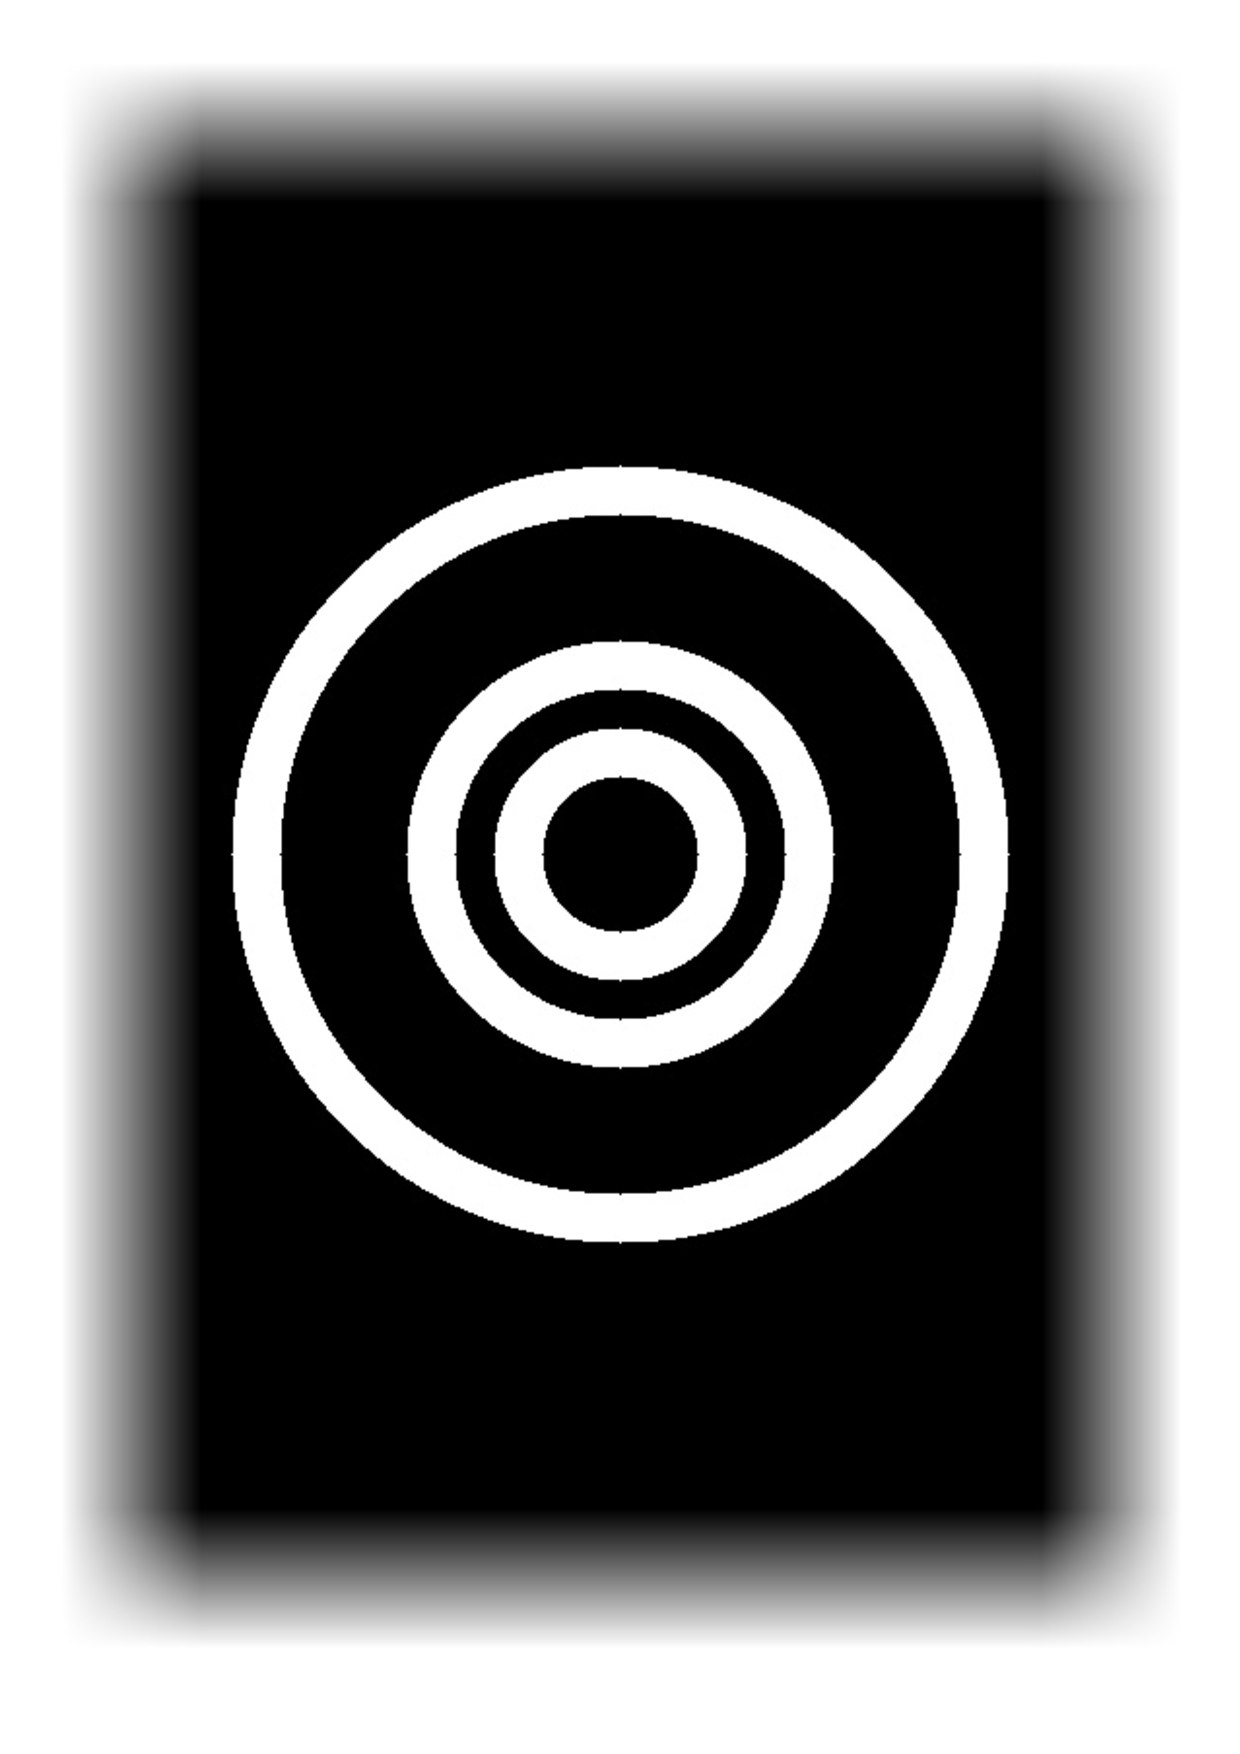
\includegraphics[width=.22\linewidth]{newconcentric_01.pdf}
  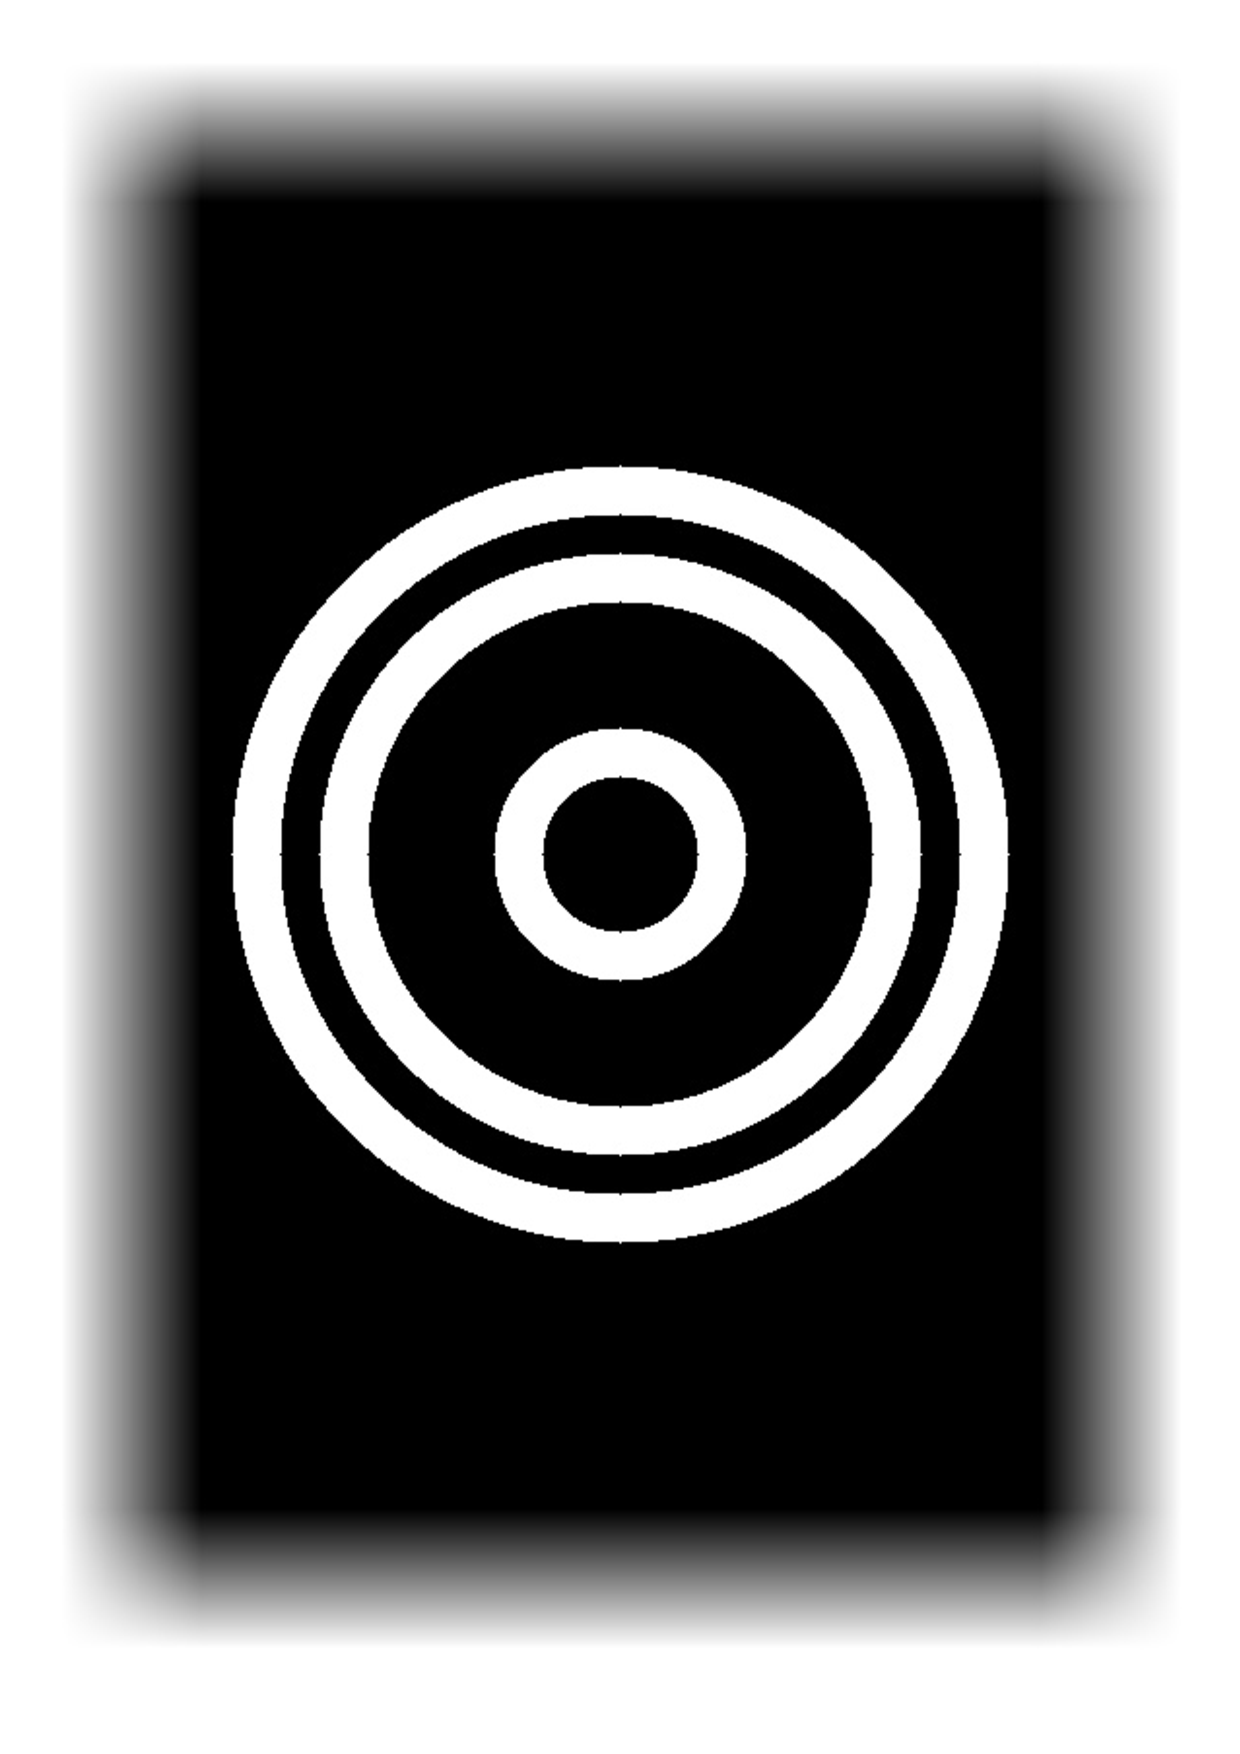
\includegraphics[width=.22\linewidth]{newconcentric_10.pdf}
  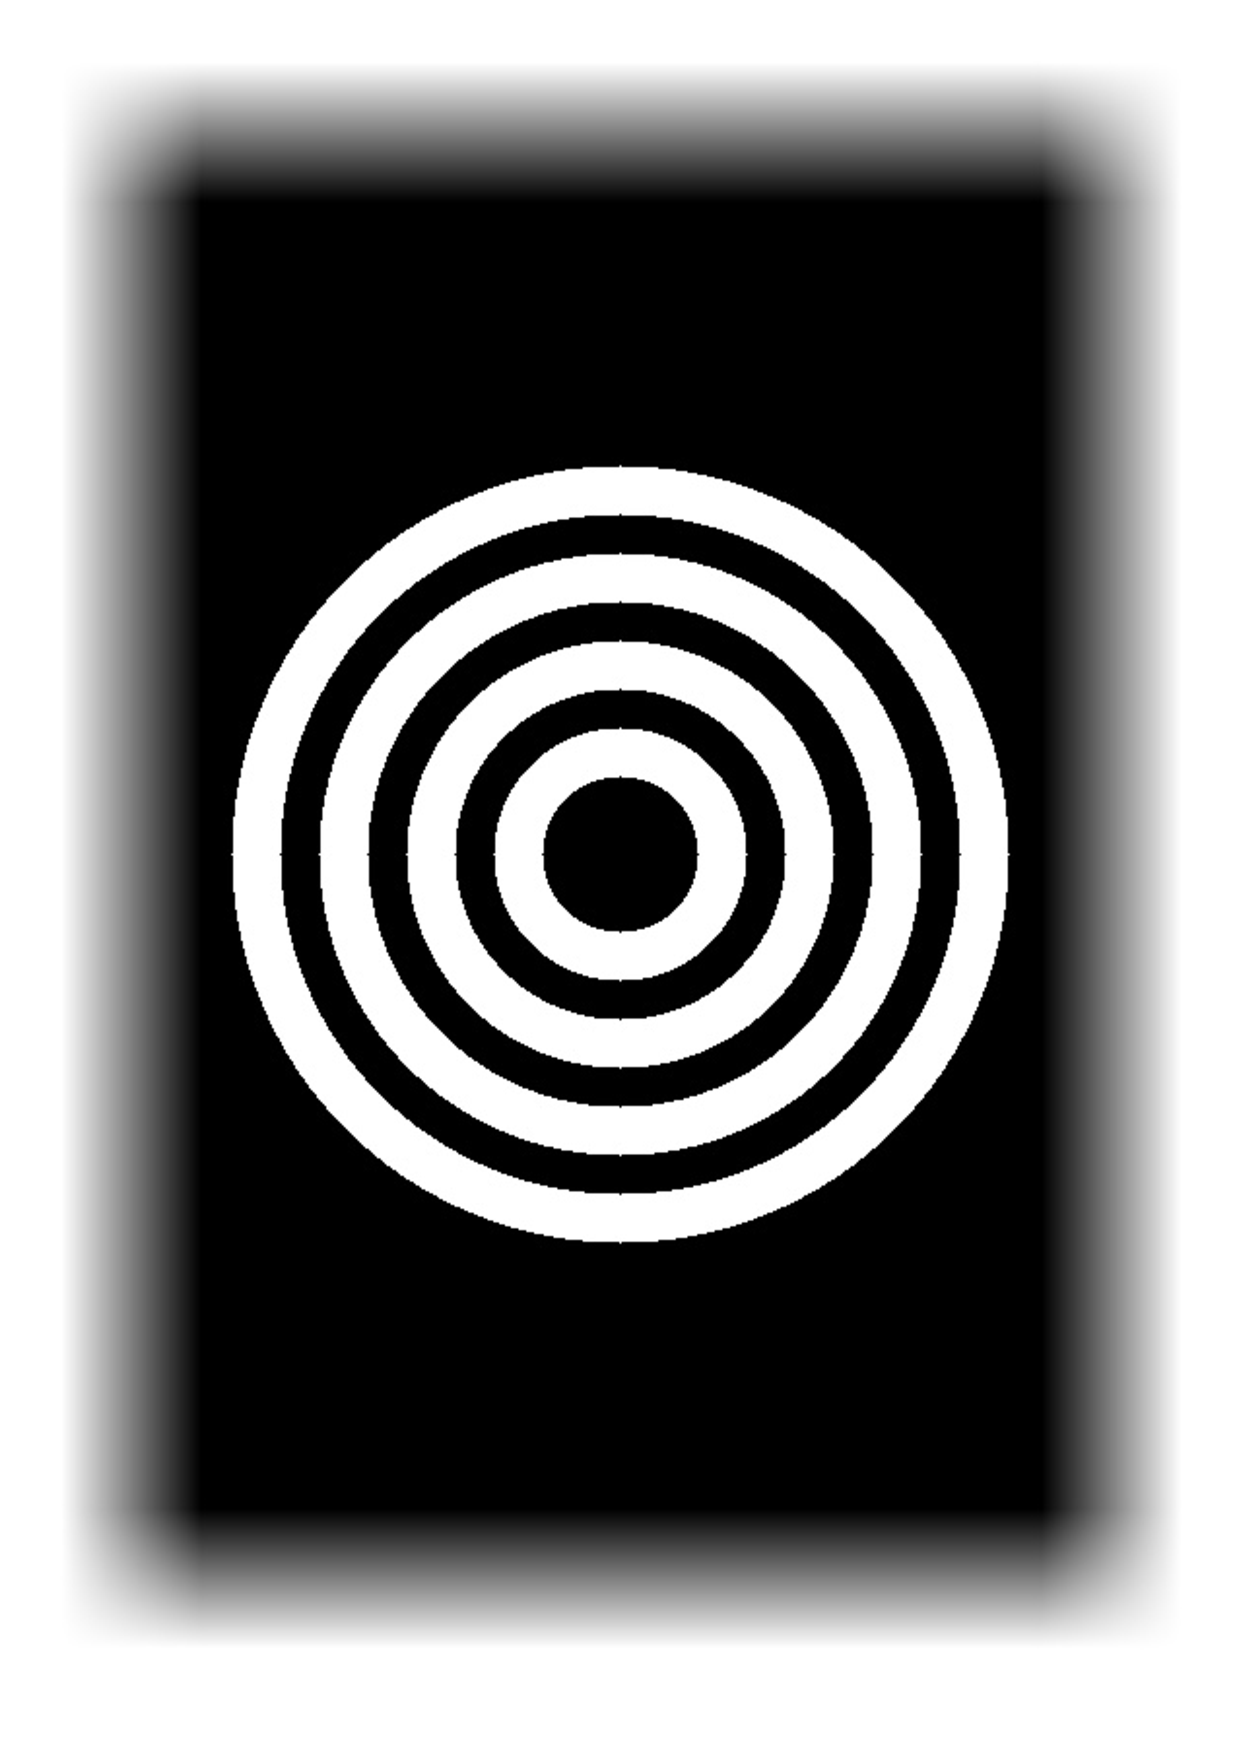
\includegraphics[width=.22\linewidth]{newconcentric_11.pdf}
  \caption{Two bit binary coded fiducials (from left to right: binary code 00,
  binary code 01, binary code 10, binary code 11)}
  \label{fig:fiducials}
\end{figure}

Depending on which ring is present or absent, the resulting binary code will
change. The number of different patterns depends on the number of bits in the
binary code. For example, if the binary code has three bits, there will be a
maximum of three rings between``marker'' rings and we end up with eight
different patterns. Figure \ref{fig:fiducials} shows two bit binary coded
fiducials. 

\subsection{Fiducial Detection Algorithm}

\begin{figure}
\centering
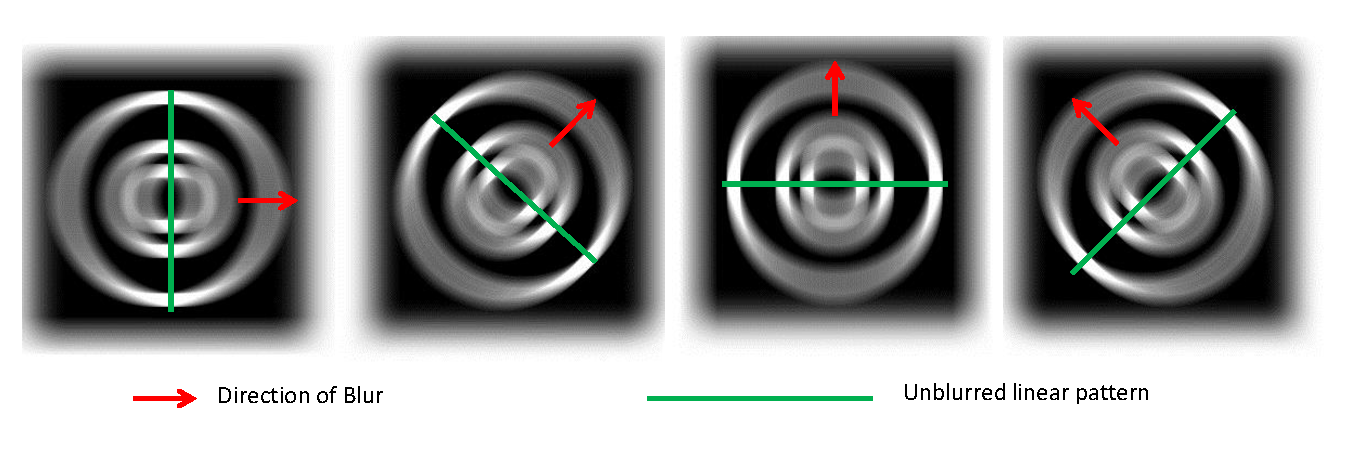
\includegraphics[width=\linewidth]{blur_direction.pdf}
\caption{Figure showing how change in blur direction changes the location of
unblurred linear pattern.}
\label{fig:blur_direction}
\end{figure}

Our fiducial detection strategy is different from \cite{NaimarkF02,Pitag13} and works
under significant amounts of blur.   As previously mentioned, our approach works
 under the assumption that the motion blur on the camera mount on the quadcopter
 can be modelled as linear motion.  This assumption about the motion blur has been shown to be
 reasonable in prior works targeting camera motion blur (e.g.~\cite{Moshe:2003,Moshe:2004}).
Under this assumption, the scene content perpendicular to the blur direction is
unaffected by the blur.  Because of our circular design, this means the
perpendicular direction can be observed as a unblurred linear pattern.  Figure
\ref{fig:blur_direction} shows an example with various motion directions.

We give a brief overview of our algorithm here and details to each step in the
following. Figure \ref{fig:overall_flow} shows the process involved in fiducial
detection process. Our detection algorithm has four steps. First, we apply a
Gabor filter (Step 1) on the image captured through AR Drone. Next, we find the
clusters of patches found in Gabor output using hierarchical clustering (Step
2). Later, we perform Principal Component Analysis (PCA) on each cluster, to
find the blur invariant direction (Step 3). The intensity profile along this
direction is found in the original image. And finally, we match this intensity
profile with training data using K-Nearest neighbor classifier (Step 4). 

\begin{comment}
Overall flow of fiducial detection algorithm can be summarised as follows:

\begin{itemize}
  \item Apply Gabor filter on input image
  \item Find connected components in Gabor output
  \item Cluster the connected components into bounding boxes
  \item Detect code in the bounding box
  \begin{itemize}
    \item Run PCA on Gabor output in bounding box
    \item Find intensity profile along first principal component passing through
    centroid
    \item Classify the detected code by training examples
    standards.
  \end{itemize}
\end{itemize}
\end{comment}

\begin{figure}[ht!]
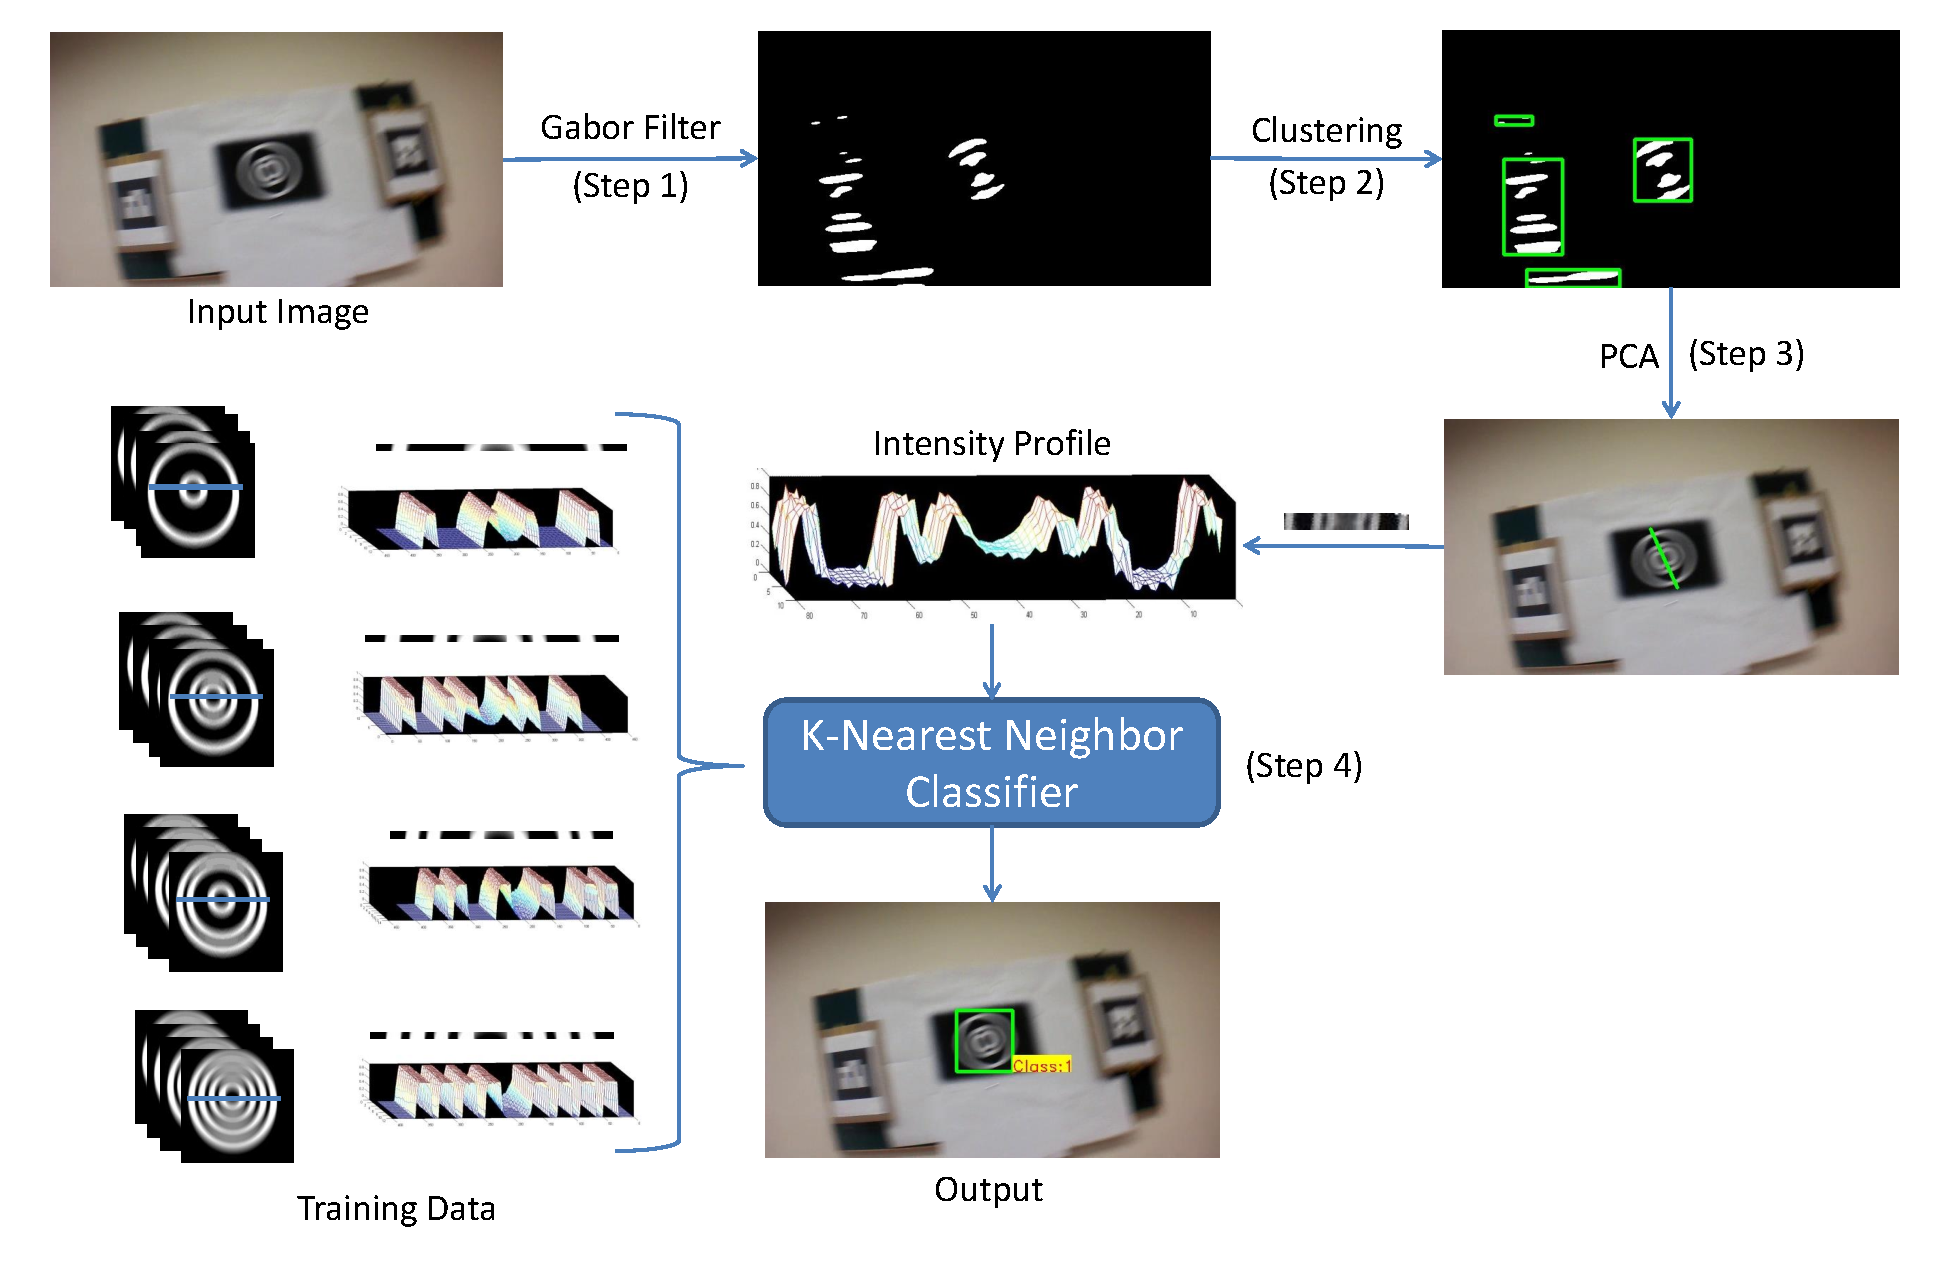
\includegraphics[width=\linewidth]{overall_flow.pdf}
\caption{The flow of our algorithm to detect and classify fiducial in the scene
captured from AR Drone. Four step process includes Gabor Filter(Step 1),
Hierarchical Clustering (Step 2), PCA (Step 3) and Classification using
K-Nearest Neighbor (KNN) classifier (Step 4). Training data for KNN classifier is gathered
offline.}
\label{fig:overall_flow}
\end{figure}

\noindent Details of each of the steps are as follows:\\
\noindent\textbf{Gabor filter}: A 2D Gabor filter is a Gaussian kernel function
modulated by a sinusoidal plane wave. It is used to find high gradient patches from the
image. In our case, it will detect blur invariant sections of the fiducials. We
have applied Gabor filter for eight different orientations ($\theta = 0, 45,
90, 135, 180, 225, 270, 315$). We have used following parameters for
creating each Gabor kernel: $\lambda = 8$, $\gamma = 0.5$, $\sigma =
0.56\lambda$, $\psi = 0 \text{(for real part)}, \pi/2 \text{(for imaginary
part)}$.
Then L2 norm of outputs along all orientations is calculated and finally L2
normed image is binarized.

\noindent\textbf{Clustering}: Connected components are found from the Gabor
output.
These connected components are then clustered in hierarchical fashion, to find
the group of closely positioned patches.

\noindent\textbf{PCA}: Principal Component Analysis is done on the clustered
Gabor output. Along first principal component, intensity profile in the original image
is found. Number of transitions in the intensity profile will give us the
number of rings.

\noindent\textbf{Classification}: Each synthetic fiducial pattern is blurred
along 36 orientations (0, 10, 20, \ldots , 350) and intensity profile along first
principal component from every output is taken as training data for that
fiducial pattern. Process of creation of training data for fiducial with
code ``01'' is depicted in Figure \ref{fig:training_data}. Test pattern is matched
against training data using K-Nearest Neighbor Classifier (K=5) to output class label.

\begin{figure}[h!]
\centering
  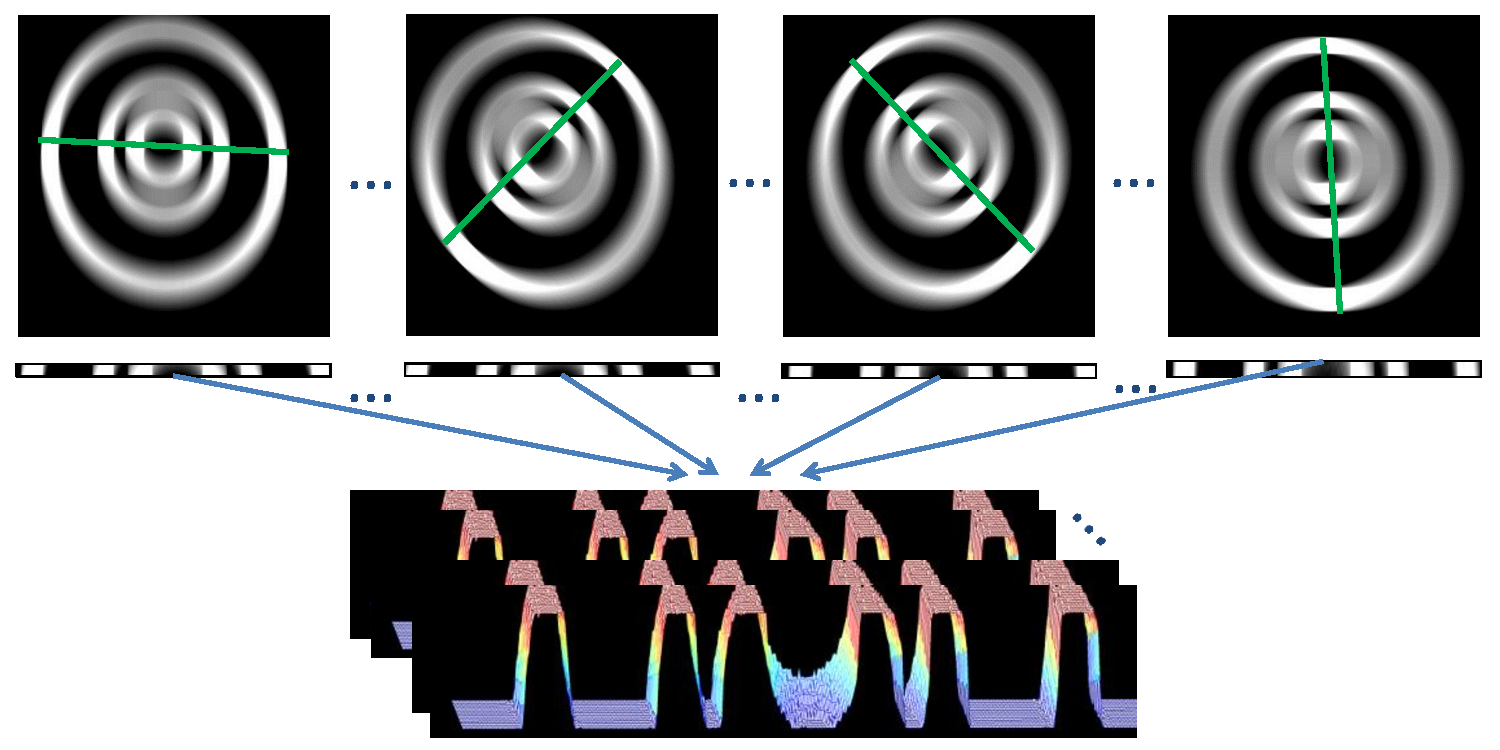
\includegraphics[width=\linewidth]{training_data.pdf}
  \caption{Process to create training data for the fiducial pattern with binary
  code ``01''. Synthetic pattern is blurred along various orientations. Gabor
  filter is applied on the blurred pattern. Intensity profile is found along the
  first principal component of the clustered Gabor output. Same process is used
  to create training data for other fiducial patterns.}
  \label{fig:training_data}
\end{figure}

To increase classification accuracy, training data for patterns having same
number of rings is grouped together; e.g., in two bit binary coded fiducial,
training data for pattern ``01'' and ``10'' will be grouped together, In three
bit binary coded fiducial, training data for pattern “001”, “010” and “100” will
form one group while training data for pattern “110”, “011” and “101” will be
in other group, etc. Now, Depending on the number of detected rings in test
pattern, it is matched against corresponding group of training data, again
using  K-Nearest Neighbor Classifier. In this way, if we detect either zero
rings or maximum possible rings in the test pattern, there will be no need to do
further classification.

\section{Experimental Validation}

We have implemented our algorithm in C++ using OpenCV library.
Experiments were performed on a PC with Intel Core i7 processor(@3.4GHz) and 4GB RAM.
Source code and data sets in this paper will be made publicly available.

Our system has been tested several image sequences captured from AR Drone
quadcopter. Each image sequence contains frames containing different fiducial
pattern. Sample output for each fiducial pattern is shown in Figure
\ref{fig:output0} -- Figure \ref{fig:output3}. Our detection process takes
around 0.3 seconds and can handle three to four frames per second.

\begin{figure}[hb!]
\begin{subfigure}{\textwidth}
\centering
  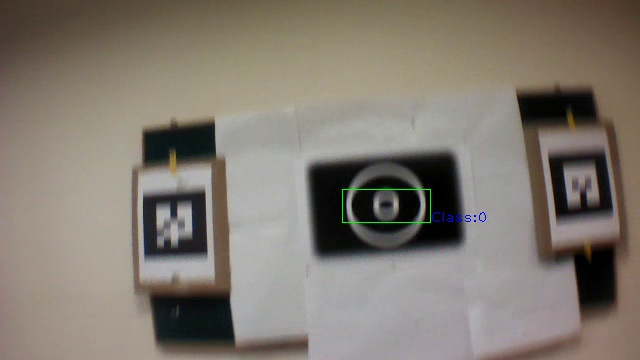
\includegraphics[width=0.48\linewidth]{output_00.jpg}
  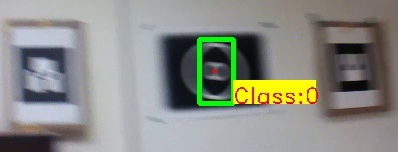
\includegraphics[width=0.48\linewidth]{new_results/output_00.jpg}
  \caption{Binary code ``00''}
  \label{fig:output0}
\end{subfigure}
\begin{subfigure}{\textwidth}
\centering
  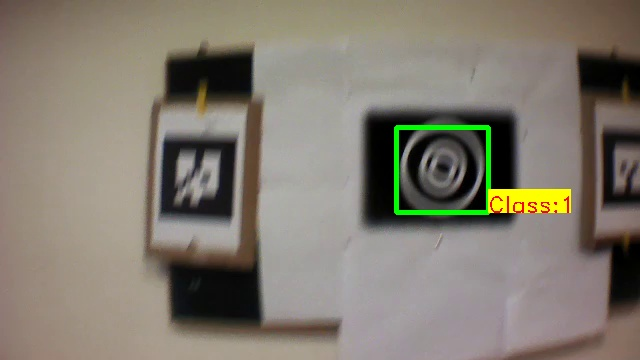
\includegraphics[width=0.48\linewidth]{output_01.jpg}
  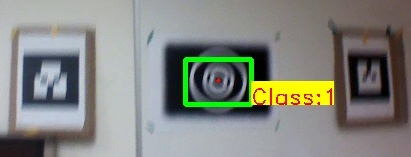
\includegraphics[width=0.48\linewidth]{new_results/output_01.jpg}
  \caption{Binary code ``01''}
  \label{fig:output1}
\end{subfigure}
\begin{subfigure}{\textwidth}
\centering
  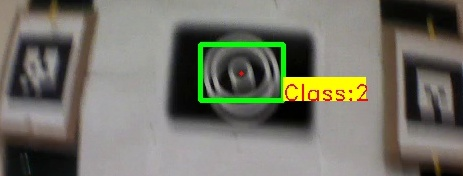
\includegraphics[width=0.48\linewidth]{output_10.jpg}
  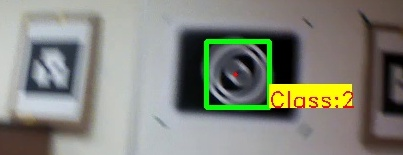
\includegraphics[width=0.48\linewidth]{new_results/output_10.jpg}
  \caption{Binary code ``10''}
  \label{fig:output2}
\end{subfigure}
\begin{subfigure}{\textwidth}
\centering
  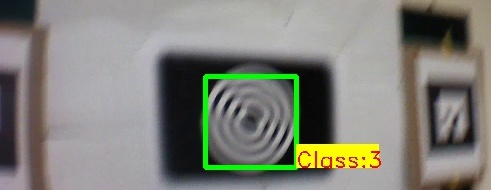
\includegraphics[width=0.48\linewidth]{output_11.jpg}
  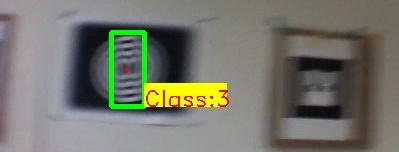
\includegraphics[width=0.48\linewidth]{new_results/output_11.jpg}
  \caption{Binary code ``11''}
  \label{fig:output3}
  \end{subfigure}
  \caption{Sample outputs for two bit binary coded fiducials on different
  datasets. Class label attached to the detected fiducial is decimal equivalent
  of the binary code embedded in the detected fiducial.}
\end{figure}

Our system has also been tested on images containing multiple fiducial patterns
in the same frame. Our algorithm successfully detected all fiducial patterns as
well as correctly classified them as shown in Figure \ref{fig:output_all}.

\begin{figure}
\centering
  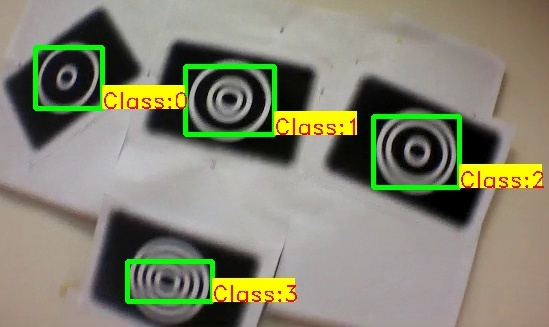
\includegraphics[width=.45\linewidth]{output_all_2.jpg}
  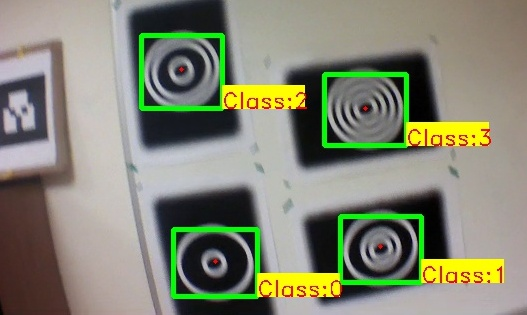
\includegraphics[width=.45\linewidth]{new_results/output_test_all1.jpg}
  \caption{Sample outputs containing all two bit binary coded fiducial patterns
  in single frame}
  \label{fig:output_all}
\end{figure}

\subsection{Comparison}
We will compare our results with standard fiducials such as ARTag. Also, we will
compare our results with Blur driven tracker(BLUT)\cite{Wu:2011}.
\subsubsection{Comparison with ARTag:}
First, we have repeated blur simulation experiment on our fiducials too, i.e.,
we have downsized our fiducial to size 150x150 and blurred it along various
orientations with different blur scales. Then, we tried to detect the patterns
using algorithm presented in earlier section. The comparison of recognition
rate is shown in Figure \ref{fig:recognition_rate}.

\begin{figure}[h!]
\centering
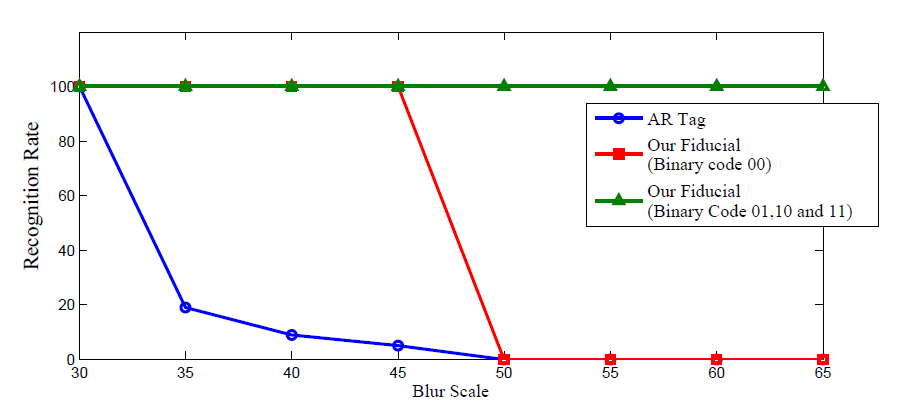
\includegraphics[width=\linewidth]{recognition_rate.png}
\caption{Comparison of recognition rate of AR Tag and our fiducials on
blur simulated data at various blur scales. It can be clearly seen that except
fiducial with binary code ``00'', our fiducial patterns are
recognised all times.}
\label{fig:recognition_rate}
\end{figure}

Later, we recorded the real data using AR Drone quadcopter. In our experimental
setup, we have kept our fiducial along with two AR Tags, to compare the
resilience of blur by each fiducial type. We have used ar\_track\_alvar, ROS
Wrapper for ALVAR library \cite{ros_alvar}, to detect AR Tags from the stream
captured through quadcopter. In each test dataset, we used different two bit
binary coded fiducial and recorded video of around two minute duration (i.e.,
around 1000 frames) The comparison of recognition rate is shown in Table
\ref{tab:recongition_accuracy}. Classification accuracy of all fiducials (ARTag
as well as ours) is almost 100\%.

\begin{table}[h!]
\caption{Comparison of recognition rate of AR Tag and our fiducials on real
data captured through AR Drone. Each row shows analysis of a test
dataset captured for our fiducial with different binary code embedded in it.
Each dataset has around 1000 frames captured in around two minutes.}
\centering
\begin{tabularx}{\textwidth}{|c|Y|Y|Y|Y|}
\cline{1-5}
\multirow{2}{*}{Test \#} & \multirow{2}{*}{Number of Frames}
&\multirow{2}{*}{Binary Code} &\multicolumn{2}{c|}{Recognition Rate (\%)} \\
\cline{4-5} & & & Our Fiducial & AR Tag\\\cline{1-5}
1 & 1205 & 00 & 86.5 &  65.6 \\ \cline{1-5}
2 & 1047 & 01 & 94.1 &  61.9 \\ \cline{1-5}
3 & 1102 & 10 &  92.74 & 62.4 \\ \cline{1-5}
4 & 1081 & 11 & 93.54 & 60.3 \\ \cline{1-5}
\end{tabularx}
\label{tab:recongition_accuracy}
\end{table}
 
\subsubsection{Comparison with BLUT:}

We have used four image sequences (consisting of around 1000 frames each) , each
one containing our different fiducial pattern, to test the performance of
BLUT\cite{Wu:2011} and compare it with our result on the same image sequence.
From top rows of Figure \ref{fig:BLUT_compare_00}-\ref{fig:BLUT_compare_11}, it
can be inferred that BLUT is able to track the fiducial when the position of
fiducial does not change too much in successive frames. Also, it can be seen
that, once BLUT looses the track of the fiducial, it is not able to recover
from that. But, our algorithm is able to track the fiducial irrespective of the
change in the position of the fiducial in the image as shown in bottom rows of Figure
\ref{fig:BLUT_compare_00}-\ref{fig:BLUT_compare_11}.

We have also found that, even if we reset the BLUT tracker after loosing track,
it looses track again after around 100 frames i.e., approximately 6 seconds.
When we checked the timestamp data from image header captured through AR Drone,
we found that, there was difference of 0.14 seconds between two successive
frames in the earlier case, which clearly suggests the dropping of frame. Also,
there were around 50 instances in 1000 frames where timestamp difference between two
successive frames was greater than 0.1 seconds. So, it is evident that
due to dropping of frames combined with unstable motion of quadcopter, tracking
through quadcopter using conventional tracking methods is not accurate.

\begin{figure}
\begin{subfigure}[b]{.19\textwidth}
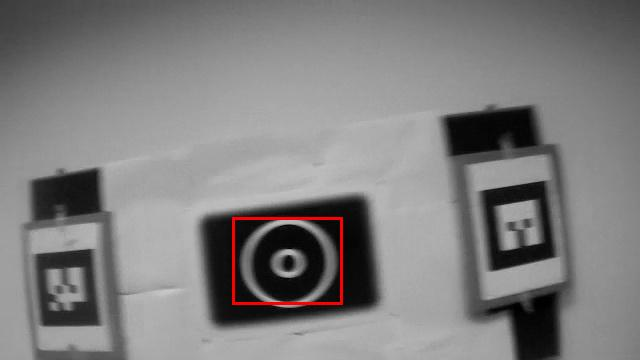
\includegraphics[width=\linewidth]{BLUT_output_00/2.jpg}
\end{subfigure}
\begin{subfigure}[b]{.19\textwidth}
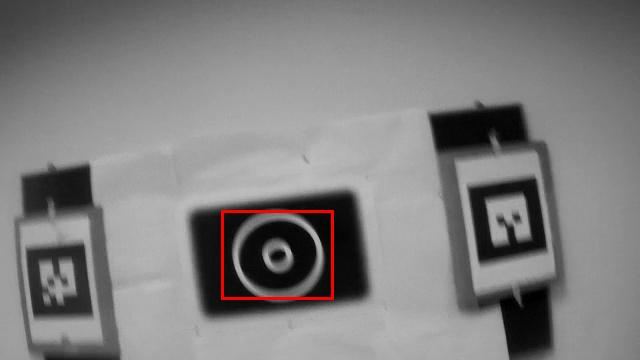
\includegraphics[width=\linewidth]{BLUT_output_00/3.jpg}
\end{subfigure}
\begin{subfigure}[b]{.19\textwidth}
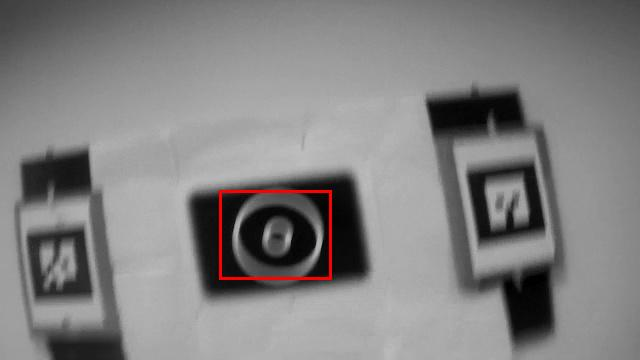
\includegraphics[width=\linewidth]{BLUT_output_00/4.jpg}
\end{subfigure}
\begin{subfigure}[b]{.19\textwidth}
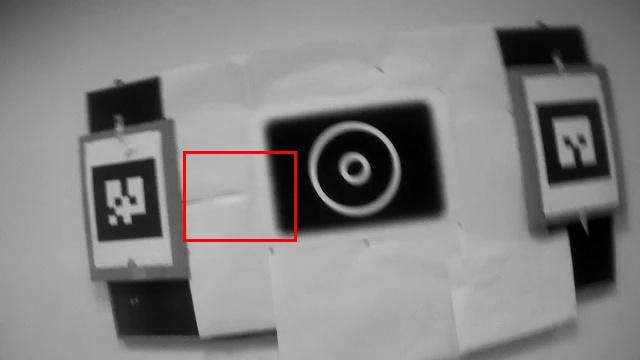
\includegraphics[width=\linewidth]{BLUT_output_00/5.jpg}
\end{subfigure}
\begin{subfigure}[b]{.19\textwidth}
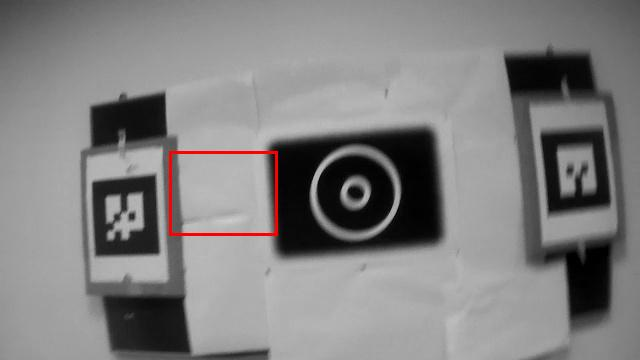
\includegraphics[width=\linewidth]{BLUT_output_00/6.jpg}
\end{subfigure}\\
\begin{subfigure}[b]{.19\textwidth}
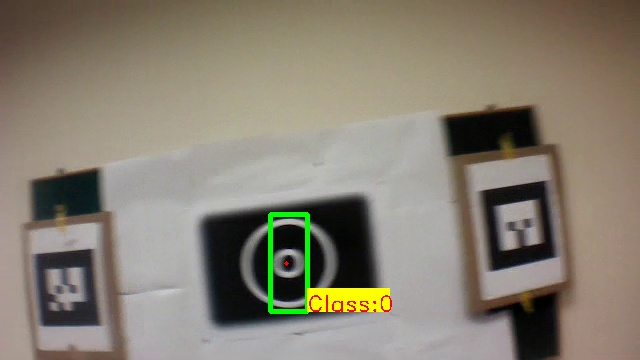
\includegraphics[width=\linewidth]{BLUT_input_00/output2.jpg}
\end{subfigure}
\begin{subfigure}[b]{.19\textwidth}
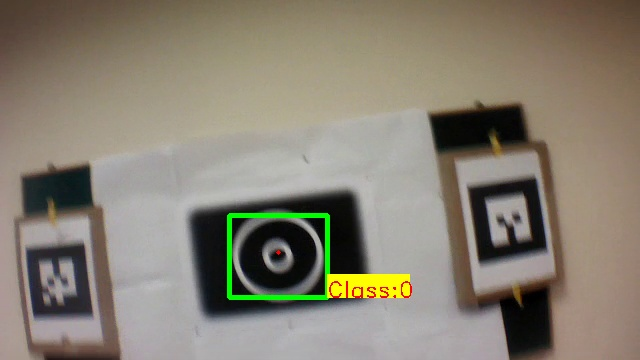
\includegraphics[width=\linewidth]{BLUT_input_00/output3.jpg}
\end{subfigure}
\begin{subfigure}[b]{.19\textwidth}
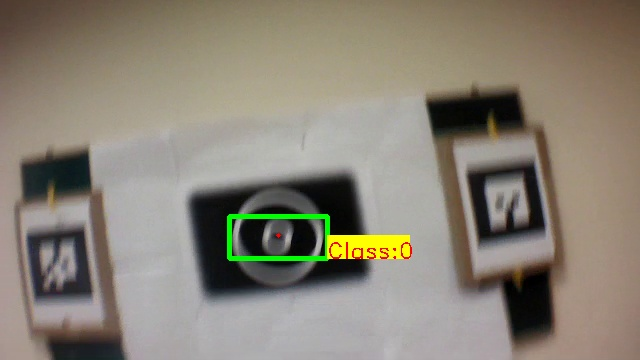
\includegraphics[width=\linewidth]{BLUT_input_00/output4.jpg}
\end{subfigure}
\begin{subfigure}[b]{.19\textwidth}
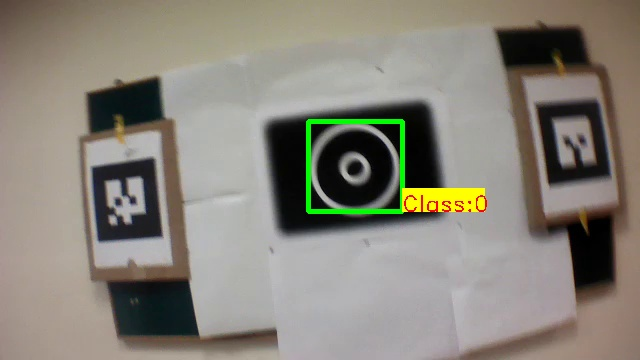
\includegraphics[width=\linewidth]{BLUT_input_00/output5.jpg}
\end{subfigure}
\begin{subfigure}[b]{.19\textwidth}
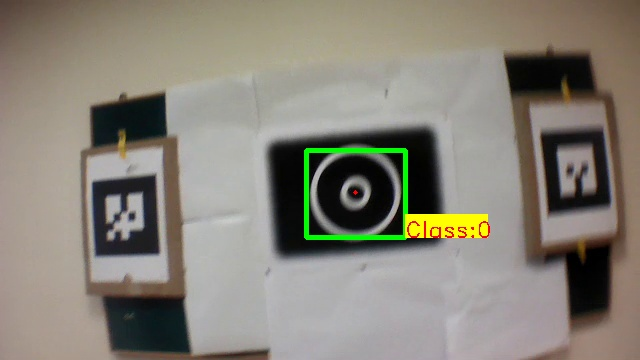
\includegraphics[width=\linewidth]{BLUT_input_00/output6.jpg}
\end{subfigure}
\caption{Top: Output of BLUT\cite{Wu:2011} on sample image sequence containing ``00''
binary coded fiducial, Bottom: Output of our algorithm on the same image
sequence. BLUT is able to track the fiducial till third frame, but from fourth
frame, BLUT looses track of the fiducial. In first three frames, size of the
fiducials is less but in fourth and fifth frame it is bigger, hinting sudden
forward movement of quadcopter.}
\label{fig:BLUT_compare_00}
\end{figure}

\begin{figure}
\begin{subfigure}[b]{.19\textwidth}
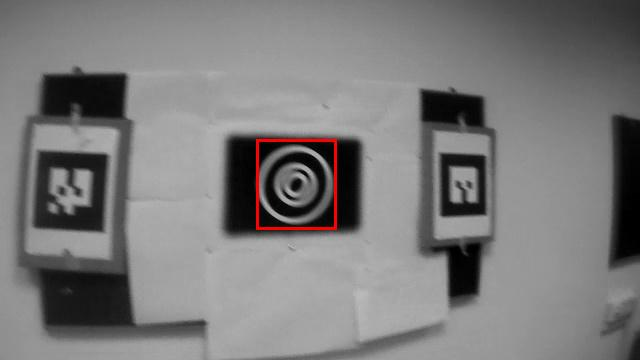
\includegraphics[width=\linewidth]{BLUT_output_01/11.jpg}
\end{subfigure}
\begin{subfigure}[b]{.19\textwidth}
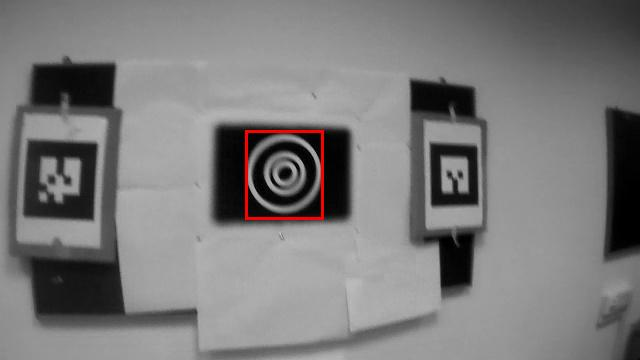
\includegraphics[width=\linewidth]{BLUT_output_01/12.jpg}
\end{subfigure}
\begin{subfigure}[b]{.19\textwidth}
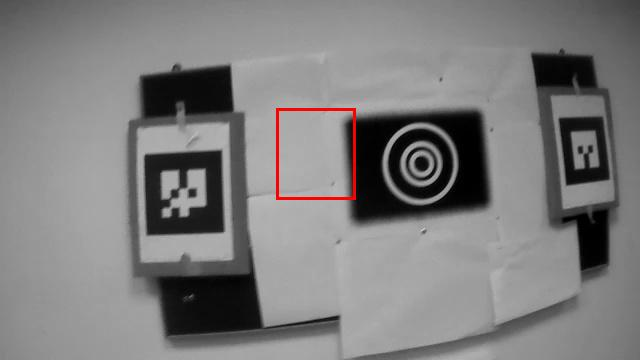
\includegraphics[width=\linewidth]{BLUT_output_01/13.jpg}
\end{subfigure}
\begin{subfigure}[b]{.19\textwidth}
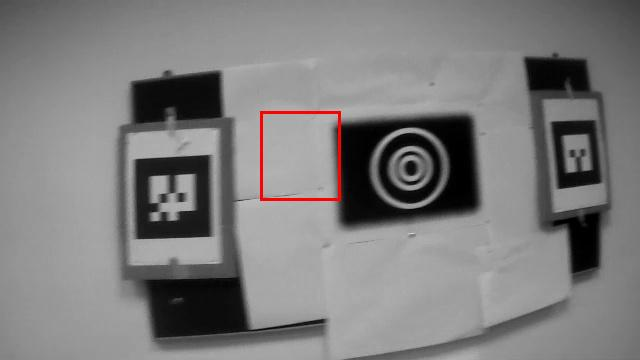
\includegraphics[width=\linewidth]{BLUT_output_01/14.jpg}
\end{subfigure}
\begin{subfigure}[b]{.19\textwidth}
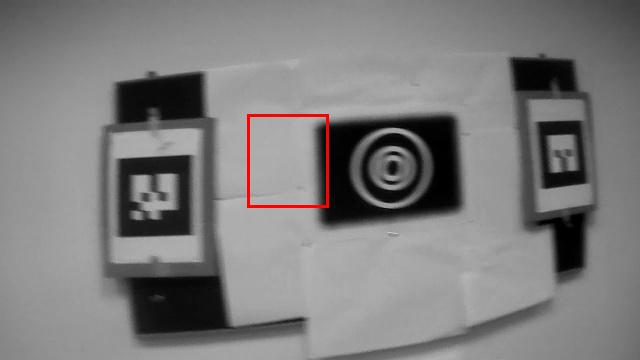
\includegraphics[width=\linewidth]{BLUT_output_01/15.jpg}
\end{subfigure}\\
\begin{subfigure}[b]{.19\textwidth}
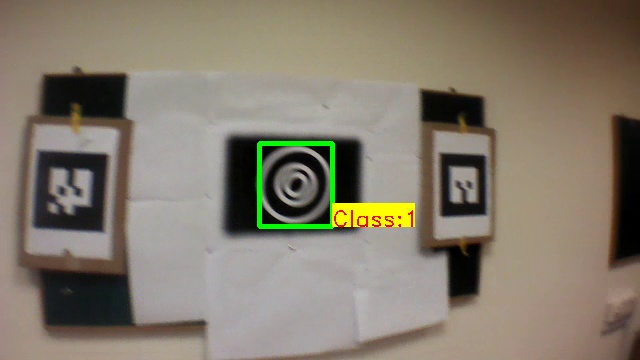
\includegraphics[width=\linewidth]{BLUT_input_01/output11.jpg}
\end{subfigure}
\begin{subfigure}[b]{.19\textwidth}
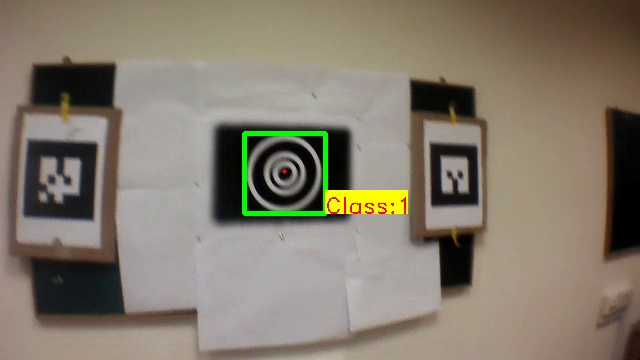
\includegraphics[width=\linewidth]{BLUT_input_01/output12.jpg}
\end{subfigure}
\begin{subfigure}[b]{.19\textwidth}
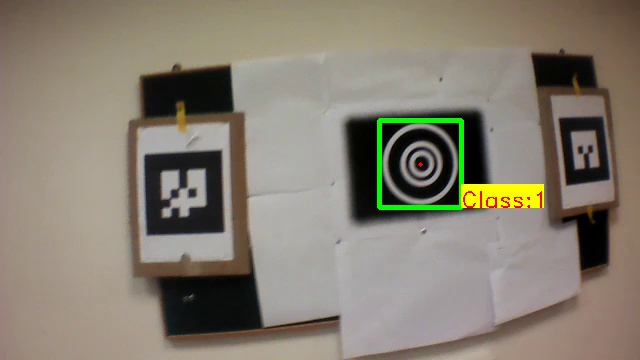
\includegraphics[width=\linewidth]{BLUT_input_01/output13.jpg}
\end{subfigure}
\begin{subfigure}[b]{.19\textwidth}
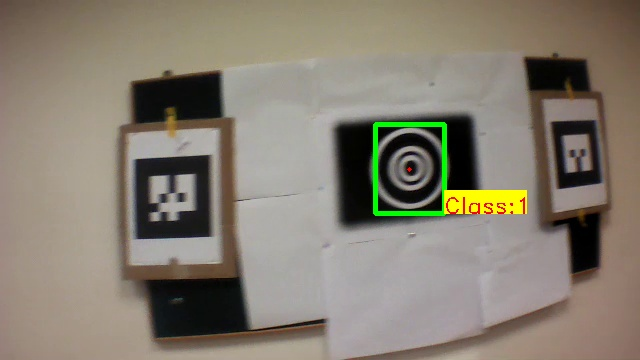
\includegraphics[width=\linewidth]{BLUT_input_01/output14.jpg}
\end{subfigure}
\begin{subfigure}[b]{.19\textwidth}
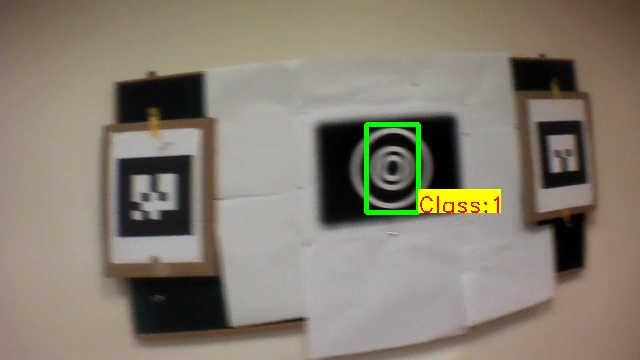
\includegraphics[width=\linewidth]{BLUT_input_01/output15.jpg}
\end{subfigure}
\caption{Top: Output of BLUT\cite{Wu:2011} on sample image sequence containing
``01'' binary coded fiducial, Bottom: Output of our algorithm on the same image
sequence. BLUT looses the track from third frame.}
\label{fig:BLUT_compare_01}
\end{figure}

\begin{figure}
\begin{subfigure}[b]{.19\textwidth}
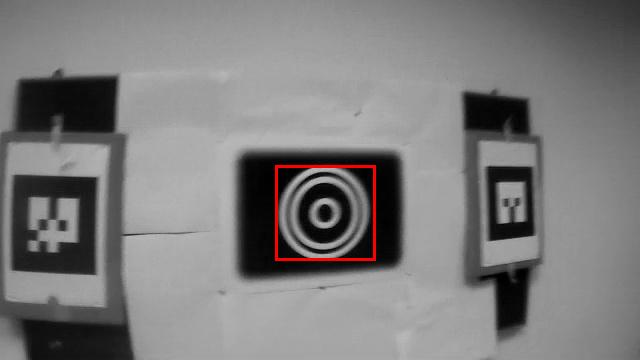
\includegraphics[width=\linewidth]{BLUT_output_10/1.jpg}
\end{subfigure}
\begin{subfigure}[b]{.19\textwidth}
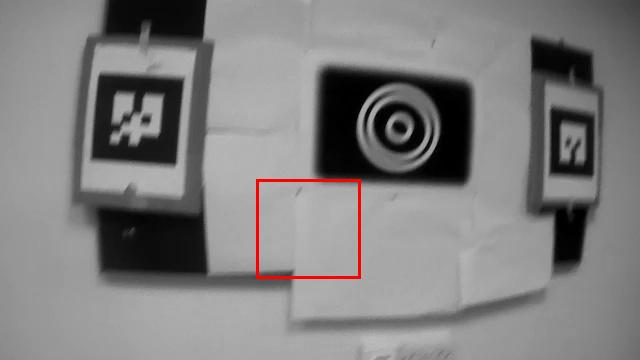
\includegraphics[width=\linewidth]{BLUT_output_10/2.jpg}
\end{subfigure}
\begin{subfigure}[b]{.19\textwidth}
\includegraphics[width=\linewidth]{BLUT_output_10/3.jpg}
\end{subfigure}
\begin{subfigure}[b]{.19\textwidth}
\includegraphics[width=\linewidth]{BLUT_output_10/4.jpg}
\end{subfigure}
\begin{subfigure}[b]{.19\textwidth}
\includegraphics[width=\linewidth]{BLUT_output_10/5.jpg}
\end{subfigure}\\
\begin{subfigure}[b]{.19\textwidth}
\includegraphics[width=\linewidth]{BLUT_input_10/output1.jpg}
\end{subfigure}
\begin{subfigure}[b]{.19\textwidth}
\includegraphics[width=\linewidth]{BLUT_input_10/output2.jpg}
\end{subfigure}
\begin{subfigure}[b]{.19\textwidth}
\includegraphics[width=\linewidth]{BLUT_input_10/output3.jpg}
\end{subfigure}
\begin{subfigure}[b]{.19\textwidth}
\includegraphics[width=\linewidth]{BLUT_input_10/output4.jpg}
\end{subfigure}
\begin{subfigure}[b]{.19\textwidth}
\includegraphics[width=\linewidth]{BLUT_input_10/output5.jpg}
\end{subfigure}
\caption{Top: Output of BLUT\cite{Wu:2011} on sample image sequence containing
``10'' binary coded fiducial, Bottom: Output of our algorithm on the same image
sequence. From second frame itself, BLUT looses the track.}
\label{fig:BLUT_compare_10}
\end{figure}

\begin{figure}
\begin{subfigure}[b]{.19\textwidth}
\includegraphics[width=\linewidth]{BLUT_output_11/2.jpg}
\end{subfigure}
\begin{subfigure}[b]{.19\textwidth}
\includegraphics[width=\linewidth]{BLUT_output_11/3.jpg}
\end{subfigure}
\begin{subfigure}[b]{.19\textwidth}
\includegraphics[width=\linewidth]{BLUT_output_11/4.jpg}
\end{subfigure}
\begin{subfigure}[b]{.19\textwidth}
\includegraphics[width=\linewidth]{BLUT_output_11/5.jpg}
\end{subfigure}
\begin{subfigure}[b]{.19\textwidth}
\includegraphics[width=\linewidth]{BLUT_output_11/6.jpg}
\end{subfigure}\\
\begin{subfigure}[b]{.19\textwidth}
\includegraphics[width=\linewidth]{BLUT_input_11/output2.jpg}
\end{subfigure}
\begin{subfigure}[b]{.19\textwidth}
\includegraphics[width=\linewidth]{BLUT_input_11/output3.jpg}
\end{subfigure}
\begin{subfigure}[b]{.19\textwidth}
\includegraphics[width=\linewidth]{BLUT_input_11/output4.jpg}
\end{subfigure}
\begin{subfigure}[b]{.19\textwidth}
\includegraphics[width=\linewidth]{BLUT_input_11/output5.jpg}
\end{subfigure}
\begin{subfigure}[b]{.19\textwidth}
\includegraphics[width=\linewidth]{BLUT_input_11/output6.jpg}
\end{subfigure}
\caption{Top: Output of BLUT\cite{Wu:2011} on sample image sequence containing
``11'' binary coded fiducial, Bottom: Output of our algorithm on the same image
sequence. BLUT lost the track from third frame. There is sudden reversal of
direction of quadcopter from third frame. In first two frames quadcopter was
going up, but suddenly it moved down in third frame.}
\label{fig:BLUT_compare_11}
\end{figure}

\section{Discussion}

\noindent\textbf{Processing Time:}~~Currently our processing time (0.3 seconds
per frame) makes it difficult to do the fiducial detection in real-time. When we have
done the code profiling, we found that Gabor filter takes most of the time (0.03
-- 0.04 seconds per orientation). As we are applying Gabor filter along eight
orientations, we should think of some optimized way to do filtering.
Alternatively, some replacement for Gabor filter needs to be find out.

\noindent\textbf{False Negatives:}~~We found that sometimes our detection
algorithm fails to recognize our fiducial with binary code ``00'' when there is
large amount of blur. This is the reason behind lower recognition rate of ``00''
coded fiducial compared to that of our other fiducial patterns. When we
investigated the problem, we found that, if there is too much blur, in Gabor
output, the innermost ring is unable to give any response along the direction
perpendicular to blur direction. This problem can be resolved by increasing
radius of innermost ring, reducing effect of blur on the innermost ring.

\noindent\textbf{Pose Estimation:}~~Currently, we are not finding the pose from
the fiducial marker. But, if we put multiple markers (at least four) in the same
scene, we may be able to find the pose. The current resolution of onboard camera
will be main hurdle to clear before we can effectively use multiple markers in
each scene.

\noindent\textbf{Number of Fiducials:}~~Currently, compared to AR Tag fiducial
markers, we are able to generate less number of fiducials. Many applications in
robotics (e.g. quadcopter navigation) may not require large number of fiducial
markers as AR Tag. Most of the time, it is sufficient to have 4-6
different fiducial patterns. Still, we may be able to generate more number of
fiducials by using color background instead of black. E.g., if we just use Red,
Green and Blue as background color, number of fiducials will be increased by
factor of three.

\section{Conclusion and Future Work}
Quadcopters are subject to quick and unstable motions that can cause significant
motion blur in the captured images. It severely affects the detection rate of
existing fiducial markers. We proposed the design of a fiducial that is robust
to motion blur. Our design of contrasting concentric rings is based on the the
observation that the direction perpendicular to the motion blur direction will
be unaffected by the blur and therefore still be recognizable. We have shown
through experimental validation that our fiducial will work under significant
amount of motion blur. When compared to popular fiducials, our fiducial can
withstand around twice the amount of blur.  Though, currently we are not able to
find the pose using single pattern, we may be able to overcome this
shortcoming by using multiple markers in single scene. Also, through faster
implementation of Gabor filter, the fiducial detection can be done in realtime.

\bibliographystyle{splncs}
\bibliography{egbib}

\end{document}

